\documentclass[xcolor=dvipsnames, notes=hide]{beamer}
%\documentclass[xcolor=dvipsnames, notes=only]{beamer}
%\documentclass[xcolor=dvipsnames]{beamer}
%\setbeameroption{show only notes}
%\usepackage{pgfpages}
%\setbeamertemplate{note page}[plain]
%\setbeameroption{show notes on second screen=right}

\usepackage[english]{babel}
\usepackage[utf8]{inputenc}
\usepackage[T1]{fontenc} % Ligaturen, richtige Umlaute im PDF

\newcommand{\backupbegin}{
	\newcounter{finalframe}
	\setcounter{finalframe}{\value{framenumber}}
}
\newcommand{\backupend}{
	\setcounter{framenumber}{\value{finalframe}}
}

\usepackage[absolute,overlay]{textpos} % textblock for figure placement

\usepackage{tabularx, booktabs}
\usepackage{amsmath}
\usepackage{blkarray, bigstrut}
\usepackage{xparse}

\usepackage[normalem]{ulem} % for \sout{}
\usepackage[ruled]{algorithm}
\usepackage{algpseudocode} 
\makeatletter
\def\BState{\State\hskip-\ALG@thistlm}
\algdef{SE}[DOWHILE]{Do}{doWhile}{\algorithmicdo}[1]{\algorithmicwhile\ #1}
\makeatother

\beamertemplatenavigationsymbolsempty
%\selectlanguage{english}
%\usepackage{biblatex}
%\bibliography{Bibliography}

\usepackage{bbm} % For mathbb{1}
\usepackage{csquotes}
\usepackage{colordvi}
\usepackage{xcolor}
%\usepackage{foiltex}

%\usepackage{enumitem}

\usepackage{tikz}
\usetikzlibrary{positioning}
\graphicspath{{/images/}}


\usetheme{CambridgeUS}
% Other valid themes
%   Antibes, Bergen, Berkeley, Berlin, Copenhagen
%   Darmstadt, Dresden, Frankfurt, Goettingen, Hannover
%   Ilmenau, JuanLesPins, Luebeck, Madrid, Malmoe
%   Marburg, Montpellier, PaloAlto, Pittsburgh, Rochester
%   Singapore, Szeged, Warsaw, boxes, default

%\usecolortheme{beetle}
%\usecolortheme{dolphin}
% Other valid color schemes
%    albatross, beaver, beetle, crane, dolphin
%    dove, fly, lily, orchid, rose, seagull
%    seahorse, whale and the one and only wolverine

%%%%%%%%%%%%%%%%%%%%%%%%%%%%%%%%
%%%%% PyCharm Color Scheme %%%%%
%%%%%%%%%%%%%%%%%%%%%%%%%%%%%%%%

%%% COLOR DEFINITIONS
\definecolor{uniBonnBlueDark}{HTML}{004F9F}
\definecolor{uniBonnYellow}{HTML}{F4B400} % lighter shades: FFDE85, FFD35C

\definecolor{pyCharmBgMain}{HTML}{2B2B2B} % RGB: 43, 43, 43

\definecolor{titleCardBg}{HTML}{CFCFEF} % former: F6511D (orange), CFCFEF (light purple) 

\definecolor{pyCharmBgSecond}{HTML}{313335}
\definecolor{pyCharmFgSecond}{HTML}{9F9FAF} % RGB: 159, 159, 175

\definecolor{pyCharmGreen}{HTML}{499C54} % RGB: 73, 156, 84
\definecolor{bfseriescolor}{HTML}{499C54}

%%% Original PyCharmColors:
%\definecolor{pyCharmBgMain}{HTML}{2B2B2B}
%\definecolor{pyCharmFgMain}{HTML}{88B1AC}
%\definecolor{pyCharmBgSecond}{HTML}{313335}
%\definecolor{pyCharmFgSecond}{HTML}{5D5F53}
%\definecolor{pyCharmGreen}{HTML}{499C54}

%%% COLOR SETTINGS
%\setbeamercolor{background canvas}{fg=pyCharmFgSecond, bg=pyCharmBgMain}
%\setbeamercolor{background}{fg=pyCharmFgSecond, bg=pyCharmBgMain}
%
%\setbeamercolor{normal text}{fg=pyCharmFgSecond,bg=pyCharmFgSecond}
%\setbeamercolor{alerted text}{fg=red}
%
\setbeamercolor{palette primary}{fg=pyCharmBgSecond, bg=white}
\setbeamercolor{palette secondary}{fg=pyCharmBgSecond, bg=white}
\setbeamercolor{palette tertiary}{fg=uniBonnBlueDark, bg=white}
%
\setbeamercolor{frametitle}{bg=titleCardBg, fg=uniBonnBlueDark} % Frametitle on every slide
\setbeamercolor{title}{fg=black, bg=titleCardBg}	% Title card slide
%
%\setbeamercolor{local structure}{fg=pyCharmGreen} % light green
%\setbeamercolor{subsection in toc}{bg=pyCharmBgMain, fg=pyCharmGreen}
%\setbeamercolor{section in toc}{bg=pyCharmBgMain, fg=pyCharmGreen}
%
%% For figure captions
%\setbeamercolor{caption}{fg=pyCharmFgSecond}
\setbeamercolor{caption name}{fg=pyCharmGreen}
%
%\setbeamertemplate{itemize item}{fg=pyCharmGreen$\blacksquare$}
%\setbeamertemplate{itemize subitem}{\color{499C54}$\blacksquare$}
%\setbeamertemplate{itemize items}[default]
%\setbeamertemplate{enumerate items}[default]

\setbeamertemplate{section in toc}{%
	{\color{pyCharmGreen} \inserttocsectionnumber.}\color{pyCharmFgSecond}~\inserttocsection}
\setbeamertemplate{subsection in toc}{%
	\hspace{1.2em}{\color{pyCharmGreen}\rule[0.3ex]{3pt}{3pt}} ~\inserttocsubsection\par}

\renewcommand{\textbf}[1]{{\bfseries\color{bfseriescolor}#1}}
%
\setbeamercolor*{palette tertiary}{bg=uniBonnBlueDark}

%%% Numbersets
\newcommand{\eye}{\mathbb{1}} % Identitiy matrix
\newcommand{\one}{\textbf{1}} % One-vector (1 1 ... 1)
\newcommand{\IN}{\mathbb{N}} % Natural numbers
\newcommand{\IR}{\mathbb{R}} % Real numbers
\newcommand{\IZ}{\mathbb{Z}} % Integers
\newcommand{\IQ}{\mathbb{Q}} % Rational numbers
\newcommand{\ID}{\mathbb{D}} % Dyadic numbers
\newcommand{\IC}{\mathbb{C}} % Complex numbers
\newcommand{\IF}{\mathbb{F}} % (Vector) Field
%\newcommand{\vA}{\mathcal{A}}
%\newcommand{\vD}{\mathcal{D}}
%\newcommand{\vB}{\mathcal{B}}
%\newcommand{\vP}{\mathcal{P}}
%\newcommand{\vJ}{\mathcal{J}}
%\newcommand{\vU}{\mathcal{U}}
%%% Basic operators
\newcommand{\IP}{\mathbb{P}} % Probability operator
\newcommand{\IE}{\mathbb{E}} % Expectation operator
\newcommand{\vF}{\mathcal{F}} % Fourier transform
%%% Distributions
\newcommand{\vN}{\mathcal{N}} % Normal distribution
\newcommand{\Bin}{\mathop{\mathrm{Bin}}} % Binomial distribution
\newcommand{\Poi}{\mathop{\mathrm{Poi}}} % Poisson distribution
%%% Others
\newcommand{\Cov}{\mathop{\mathrm{Cov}}} % covariance
\newcommand{\co}{\mathop{\mathrm{co}}} % covariance
\newcommand{\Var}{\mathop{\mathrm{Var}}} % variance
\newcommand{\norm}[1]{\left\lVert#1\right\rVert} % norm
\newcommand{\var}[1]{{\ttfamily#1}} % variable
\newcommand{\tr}{\mathop{\operatorname{tr}}} % trace
\newcommand{\rk}{\mathop{\operatorname{rk}}} % rank
\newcommand{\diag}{\mathop{\operatorname{diag}}} % diagonal
\renewcommand{\vec}[1]{\bm{#1}} % vector
\newcommand{\mat}[1]{\bm{#1}} % matrix
\newcommand{\ten}[1]{\bm{\mathcal{#1}}}
\newcommand{\inv}[1]{#1^{-1}} % inverse
\newcommand{\trn}[1]{#1^\intercal} % transpose
\newcommand{\opt}[2]{#1 \trn{#2}} % outer product
\newcommand{\ipt}[2]{\trn{#1} #2} % inner product
\newcommand{\angles}[2]{\langle #1, #2 \rangle} % scalar product
\newcommand{\Angles}[2]{\bigl \langle #1, #2 \bigr \rangle} % big scalar product
\newcommand{\st}{\operatorname{s.\!t.}} % 'such that'
%%% Stacked symbols
\newcommand{\amin}[1]{\operatorname*{argmin}_{#1}}
\newcommand{\amax}[1]{\operatorname*{argmax}_{#1}}
\newcommand{\sign}{\mathop{\mathrm{sign}}}
\newcommand{\eqex}{\mathop{\stackrel{!}{=}}}
\newcommand{\geex}{\mathop{\stackrel{!}{\ge}}}
\newcommand{\leex}{\mathop{\stackrel{!}{\le}}}
\newcommand{\softmax}{\operatorname*{softmax}}
%%% Table colors
\newcommand\cellr{\cellcolor{red!20}}
\newcommand\cellg{\cellcolor{green!10}}
\newcommand\cellb{\cellcolor{blue!10}}
\newcommand\cello{\cellcolor{orange!10}}
%%% Sets
\newcommand{\set}[1]{\{{#1}\}}
\newcommand{\Set}[1]{\big\{{#1}\big\}}
\newcommand{\BigSet}[1]{\Big\{{#1}\Big\}}
%%% Multisets
\newcommand{\mset}[1]{\{\mskip-5mu\{{#1}\}\mskip-5mu\}}
\newcommand{\Mset}[1]{\big\{\mskip-5mu\big\{{#1}\big\}\mskip-5mu\big\}}
\newcommand{\BigMset}[1]{\Big\{\mskip-5mu\Big\{{#1}\Big\}\mskip-5mu\Big\}}
%%% Footnote
%\deffootnote{1.5em}{1em}{\makebox[1.5em][l]{\thefootnotemark}}

%%% LOGO PLACEMENT
\addtobeamertemplate{frametitle}{}{%
	\begin{tikzpicture}[remember picture,overlay]
	\node[anchor=north east,yshift=-3pt] at (current page.north east) {
		
\includegraphics[height=0.8cm]{images/UNI_Bonn_Logo_Standard_RZ_XL.png}
		
\includegraphics[height=0.8cm]{images/AG_logo_hp_70x70.png}
	};
	\end{tikzpicture}}
%\addtobeamertemplate{frametitle}{}{%
%	\begin{tikzpicture}[remember picture,overlay]
%	\node[anchor=north east,yshift=-9pt] at (current page.north east) {
%		
\includegraphics[height=0.8cm]{images/UNI_Bonn_Logo_Standard_RZ_XL.png}
%		
\includegraphics[height=0.8cm]{images/AG_logo_hp_70x70.png}
%	};
%	\end{tikzpicture}}
% !Tex spellceck = en_US

\title[MA Seminar Talk - Progress]{
	\centering
	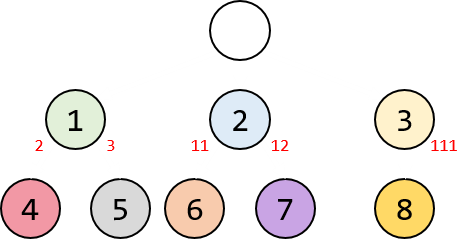
\includegraphics[width=0.3\textwidth]{images/WLLT}\\
	Master Thesis Seminar Talk	
}
%\title[MA Seminar Talk - Progress]{Master Thesis Seminar Talk}
%\titlegraphic{
%	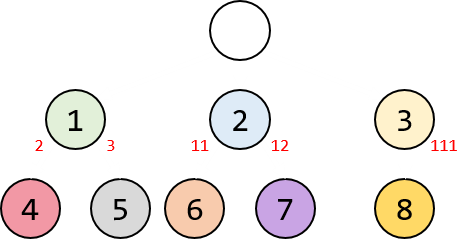
\includegraphics[width=0.2\textwidth]{images/WLLT}
%}
\subtitle{Progress Update}
\author[F. Beaumont]{Fabrice Beaumont}
\institute[]{Department of Information Systems and Artificial Intelligence - \textbf{Dr. Pascal Welke}}
\date{14. September 2022}

\newcommand{\figureWidth}{7cm}
\newcommand{\figureHorizontal}{2cm}
\newcommand{\figureVertical}{5cm}
\begin{document}


\begin{frame}
	\titlepage
\end{frame}

%%%%%%%%%%%%%%%%%%%%%%%%%%%%%%%%%%%%%%%%%%%%%%%%%%%%%%%%%%%%%%%%%%%%%%%%%
\section{Overview}

\begin{frame}
\frametitle{Progress Update} \vspace{-1cm}
	\begin{itemize}
		\item[]
		\item Implementation of all major code components completed: \newline
		\begin{itemize}
			\item Reading da TU \textbf{Dataset}, cleaning and converting it \newline
			\item Constructing a \textbf{WLLT} (ability to expand it at will) with edge weights \newline
			\item A EdgeWeightLearner-\textbf{Interface} and classes to conveniently \textbf{evaluate} the quality of the resulting clustering \newline
		\end{itemize}
		\item[]
	\end{itemize}
\end{frame}

\begin{frame}
\frametitle{Current state} \vspace{-1cm}
\begin{itemize}	
	\item Discarded the idea of \textbf{shifting weights}/\textbf{keeping} the total weight sum.\newline
	\item \textcolor{orange}{Fine-tuning} a \textbf{\enquote{DefaultLearner}}, inheriting from 
	the interface\\
	\textit{Previous goal}: Finish one version. Then code other implementations of the interface\\
	\textit{Actual situation}: Making the Default Learner more and more parameterized	
\end{itemize}
\end{frame}


%%%%%%%%%%%%%%%%%%%%%%%%%%%%%%%%%%%%%%%%%%%%%%%%%%%%%%%%%%%%%%%%%%%%%%%%%
\section{Method}


\begin{frame}
\frametitle{Example of the whole procedure}
\begin{tikzpicture}[remember picture, overlay]
\node[right] at (current page.west) 
{
	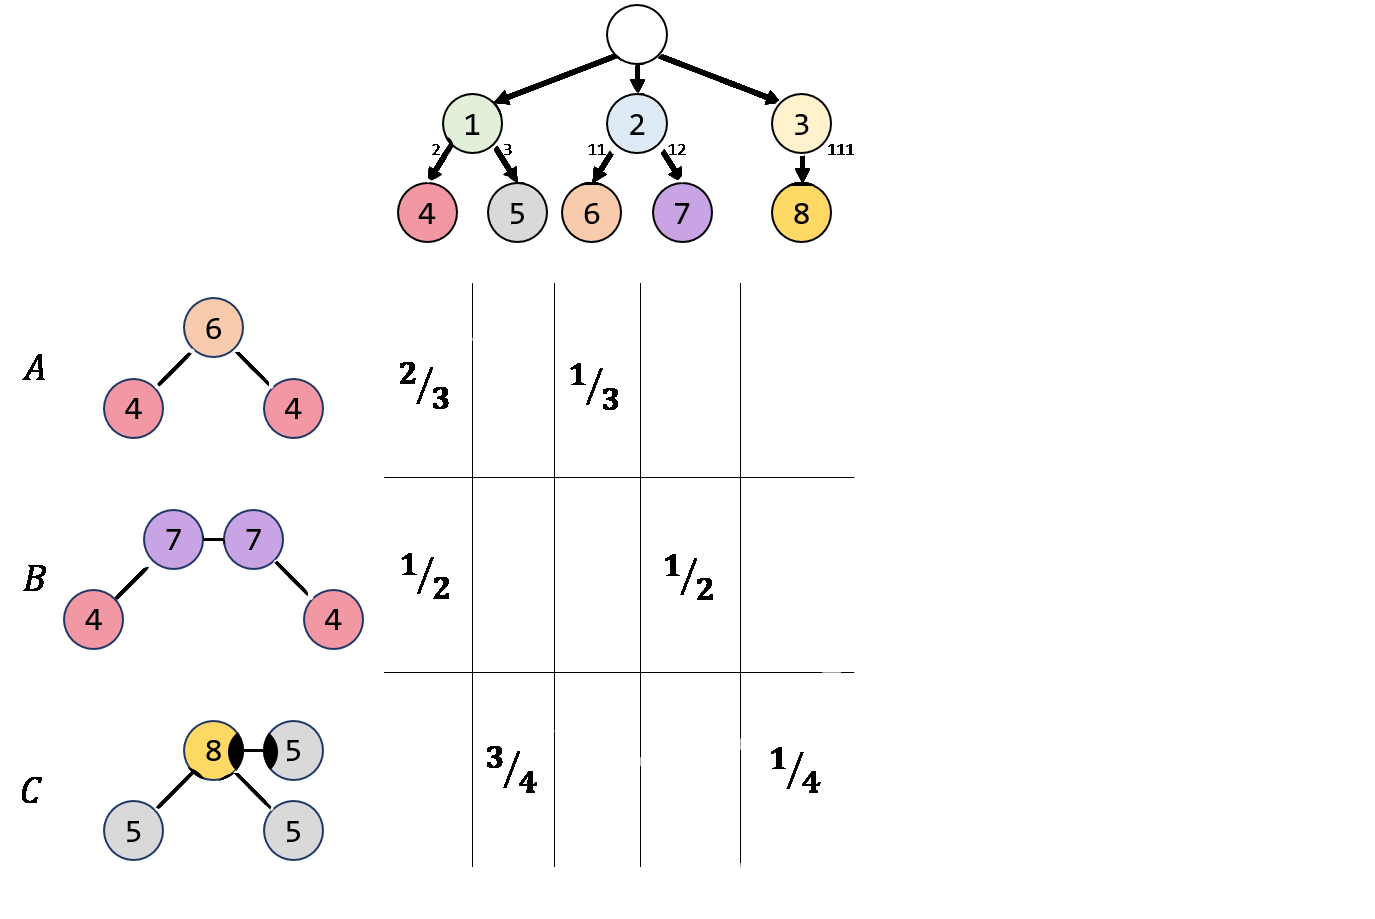
\includegraphics[width=0.9\textwidth]{images/Graphs7}
};
\end{tikzpicture}
\begin{columns}[T]%beamer
	\column{0.7\textwidth}
	% blank
	\column{0.3\textwidth}
	\textbf{Tree metric}:\\
	$\begin{array}{ccccc}
	\ \ \; \textit{4} & \textit{5} & \textit{6} & \textit{7} & \textit{8}
	\end{array}$\\
	$
	\left(		
	\begin{array}{ccccc}
	\cdot & 2 & 4 & 4 & 4 \\
	& \cdot & 4 & 4 & 4 \\
	&   & \cdot & 2 & 4 \\
	& \upuparrows & & \cdot & 4\\
	&   &   &   & \cdot
	\end{array}
	\right)
	$\\
	\textbf{Wasserstein Dist.}:\\
	$\mathcal{W}_{t}(A,B) = \frac{4}{3}$\\
	$\mathcal{W}_{t}(A,C) = 3$\\
	$\mathcal{W}_{t}(B,C) = 3$\\
\end{columns}
\vspace{0.5cm}
$d_{\text{WLLT}}(B,C) = 2*\frac{2}{4} + 4*\frac{1}{4} + 4*\frac{1}{4} = \frac{12}{4} = 3$
\end{frame}

\begin{frame}
\frametitle{Example of the whole procedure}	
\begin{columns}[T]%beamer
\column{0.5\textwidth}
\centering		
\textit{Local update} $P_{7,8}$:
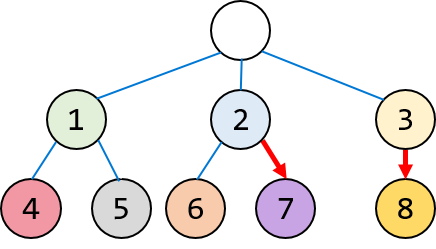
\includegraphics[width=0.8\textwidth]{images/WLLTUpdateEnds}
\textit{Weighted path update} $P_{7,8}$:
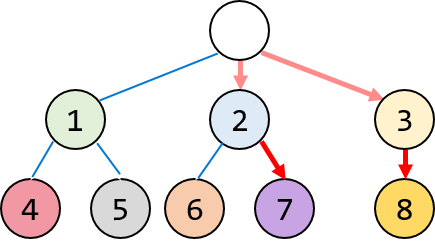
\includegraphics[width=0.8\textwidth]{images/WLLTUpdatePath}
\column{0.5\textwidth}
\begin{tikzpicture}[remember picture, overlay]
\node[left] at (current page.east) [xshift=2.5cm, yshift=-0.5cm] 
{
	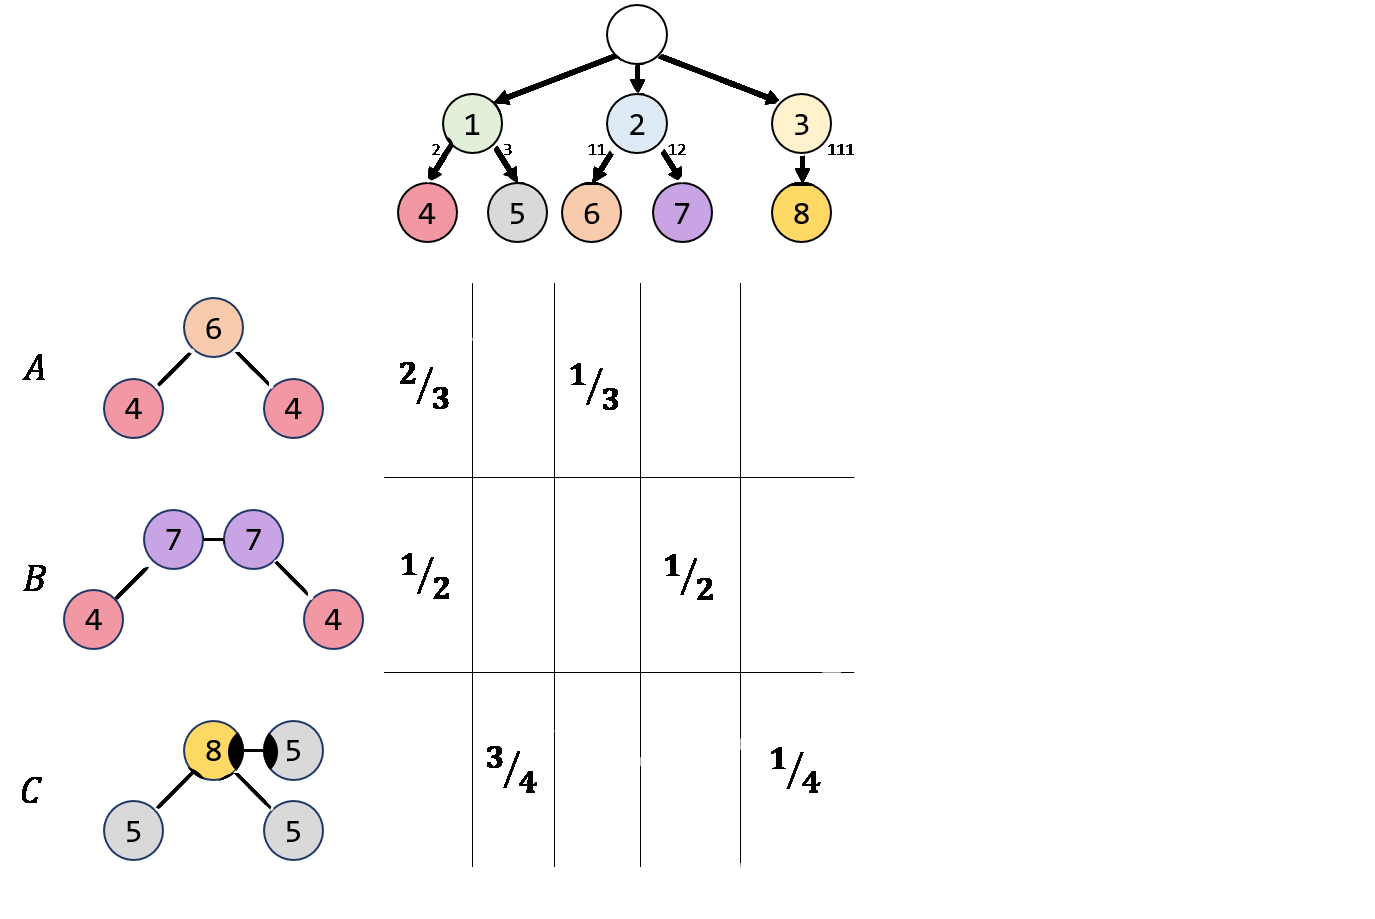
\includegraphics[width=1.2\textwidth]{images/Graphs7}
};
\end{tikzpicture}
\end{columns}
\end{frame}


%%%%%%%%%%%%%%%%%%%%%%%%%%%%%%%%%%%%%%%%%%%%%%%%%%%%%%%%%%%%%%%%%%%%%%%%%
\section{Results}

\begin{frame}
\frametitle{Implementation of the Default Learner}
	\begin{itemize}
		\item Initialize all edge weights as $1.0$
		\item Compute the \textit{Tree Wasserstein Distance}\footnote{Normalized weighted distance between their wl-label histograms.} between two graphs
		\item Select a \textbf{batch}, with \textbf{equal distributions} between all classes		
		\item Pic the \textbf{$n$} highest differences in the weighted difference vector \footnote{Most expensive earth that had to be moved.} (Option: Leaves-only)
		\item Update rule:
		\[ w^\prime = w + \lambda \Delta w\]
	\end{itemize}
\end{frame}

\begin{frame}
\frametitle{Implementation of the Learner - Update Rule}
\begin{itemize}
	\item Update rule:
	\begin{align*}
		w^\prime &= w + \lambda \Delta w \\
		&= w + \lambda \big( p_{\text{pull/push}} \ c_{\text{imba}} \ w \big)
	\end{align*}
	 
	Where:
	\begin{itemize}
		\item Learning rate $\lambda$
		\item Push-Pull-Factor:\\
		$p_{\text{pull/push}} =\begin{cases}
		+\textcolor{bfseriescolor}{p_{\text{push}}} & \text{different class}\\
		-\textcolor{bfseriescolor}{p_{\text{pull}}} & \text{same class}
		\end{cases}$
		\item Class sample imbalance factor:\\
		$c_{\text{imba}}$ account for the fact, that when selecting two samples the probability to have two samples from the same class (pulling) is lower than having two samples from different classes (pushing).
%		boils down to
%		There are 
%			(nm)(n-1)
%		possibilities to draw to samples from the SAME class. 
%		('(nm)' for any ample and '(n-1)' for the next sample in the same class.)
%		
%		There are 
%			(nm)(mn-n)  = (nm)n(m-1)
%		possibilities to draw to samples from DIFFERENT classes. 
%		('(nm)' for any ample and '(mn-n)' for the next sample from all samples, except the whole class of the first sample.)
%		
%		Since both products contain the factor (nm), we drop it by scaling. 
%		Thus we get the following factors as return values:
%		
%		#SameClass:     n-1
%		#DiffClass:     n(m-1)
%		Factor for samples in the same class:       #DiffClass / #SameClass
%		Factor for samples in different classes:    #SameClass / #DiffClass
	\end{itemize}
	\item[] 
\end{itemize}
\end{frame}

\begin{frame}
	\frametitle{Current todos / Outlook}
	\begin{itemize}
		\item[?] Why are the plots for MUTAG class -1 often zero? Is there an indexing error?\\
		(E.g. Max Intra Cl Dist C-1)
		\item[?] Why are the mean weights of mid-layers changing equally? Plotting error, update error or graph structure?
		\item[?] Why are weights in other layers changing when setting to \enquote{only-leaves}
		\item[?] Why is so few weight added? Is the balance factor correct?
		\item[!] Switch to go from relative to absolute push/pull factors
		\item[!] How to deal with different batch sizes
		% Fix the LEARNER_CONFIG updates
		% Refactoring
	\end{itemize}
\end{frame}

%%%%%%%%%%%%%%%%%%%%%%%%%%%%%%%%%%%%%%%%%%%%%%%%%%%%%%%%%%%%%%%%%%%%%%%%%
\section{End}

\begin{frame}[c]
	\centering %\Huge
	\begin{huge}
		\emph{Thank you all for listening.}\\
	\end{huge}
	\vspace{2 cm}
	I will be happy to answer any \textbf{questions} and\\
	hear your \textbf{comments}.
\end{frame}

%%%%%%%%%%%%%%%%%%%%%%%%%%%%%%%%%%%%%%%%%%%%%%%%%%%%%%%%%%%%%%%%%%%%%%%%%
\appendix
\section{Appendix}



\begin{frame}[noframenumbering]
\frametitle{Example of the whole procedure}	
\begin{columns}[T]%beamer
	\column{0.5\textwidth}
	\centering
	\textbf{Current clustering:}\\
	\vspace{0.5cm}
	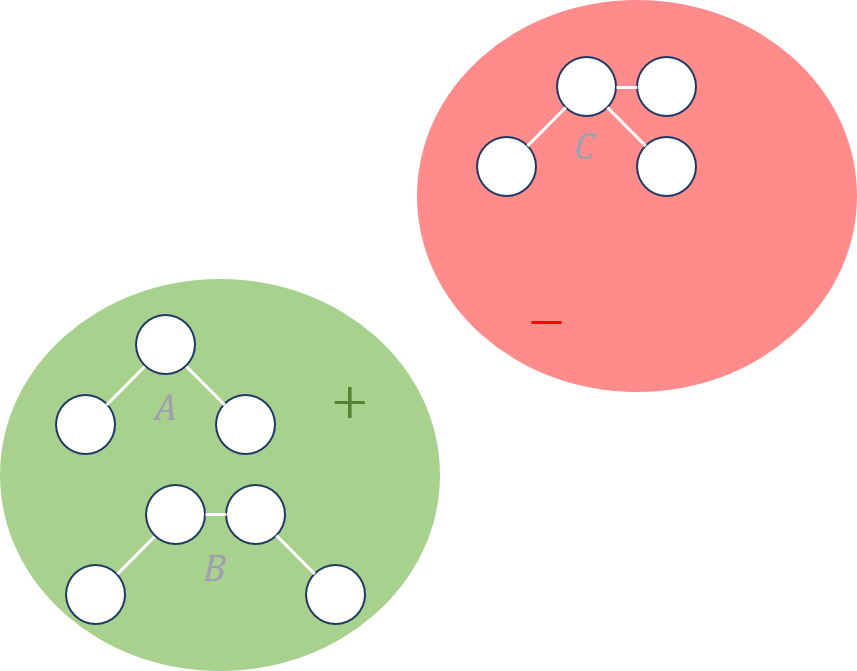
\includegraphics[width=0.8\textwidth]{images/Classification1}
	\column{0.5\textwidth}
	\centering
	\textbf{Target clustering:}\\
	\vspace{0.5cm}
	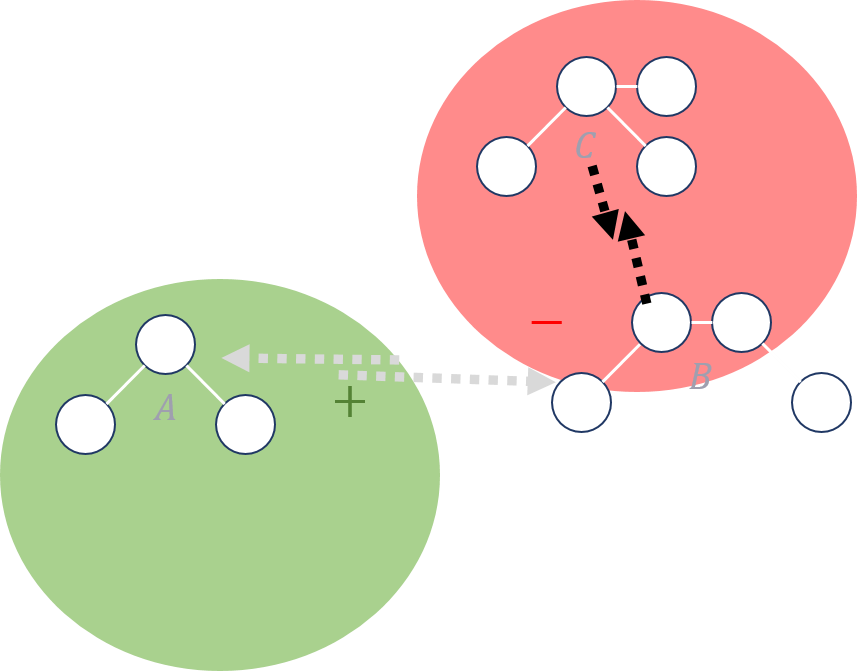
\includegraphics[width=0.8\textwidth]{images/Classification2}
\end{columns}
\vspace{0.5cm}
Idea: Reduce distance between $B$ and $C$, by updating the edge weights.
\end{frame}

\begin{frame}[noframenumbering]
	\frametitle{Preparation of the performance comparison}	
	\begin{figure}
		\centering
		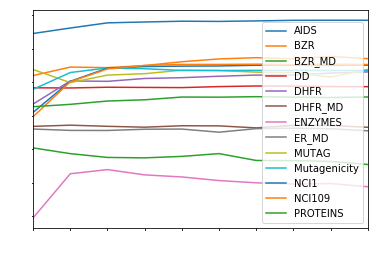
\includegraphics[width=0.6\linewidth]{images/plot_whiteText}
		\caption{Classification accuracies on databases using Weisfeiler-Lehman.}
		\label{fig:plot}
	\end{figure}
	\tiny{\texttt{grakel.kernels.\textbf{WeisfeilerLehman}(n\_iter=[1-10], base=grakel.kernels.VertexHistogram, normalize=True)}}\\
	\tiny{\texttt{grakel.utils.\textbf{cross\_validate\_Kfold\_SVM}(K, y, n\_iter=10)}}

\end{frame}


\begin{frame}[noframenumbering]
\frametitle{Implementation road-map 1/2}
\begin{itemize}
	\item \textbf{WLLT Construction}:
		\begin{itemize}
			\item Write to file and read from file. Construct WL-iteration based.
			\item All weights \textit{equal}.
			\item (\textit{Random} initial weights.)
			\item (Use \textit{a priori} knowledge.)
		\end{itemize}
	\item[]
	\item \textbf{Wasserstein-Distance feedback}:
		\begin{itemize}
			\item \enquote{Biggest pile of dirt}. 
			(\enquote{Smallest}, to increase the distance.)
			\item Distribution proportional to the pile size.
			\item Distribution proportional to the cost of moving the pile size.
		\end{itemize}	
\end{itemize}	
\end{frame}

\begin{frame}[noframenumbering]
\frametitle{Implementation road-map 2/2}
\begin{itemize}
	\item \textbf{Update rule}:
	\begin{itemize}
		\item Value:
		\begin{itemize}
			\item Constant $\lambda$.
			\item \textit{Gradient descent}.
		\end{itemize}
		\item Location:
		\begin{itemize}
			\item \textit{Local}: Only update the first and last edge weights of the connecting path.
			\item \textit{Weighted path}: Update all edge weights on the path, with less magnitude for edges closer to the root.
			\item \textit{Path}: Update all edges on the path.
			\item \textit{Global}: Update all edges, related to all occurring labels.
		\end{itemize}
	\end{itemize}		
\end{itemize}	
\end{frame}

\end{document}